
\begin{frame}{\citetitle{MarcoNuno_Revista_2020_06_00} \footnotemark (1)}
\begin{block}{Sistema de Monitoreo de Aprendizaje Remoto } 

Con la reciente pandemia, se detectan problemas con el seguimiento del aprendizaje:

	\begin{itemize}
		\item No es posible determinar si el estudiante es quien realiza las tareas
		\item No hay certeza de que tanto tiempo el estudiante dedica a ciertas tareas
	\end{itemize}

Se propone una herramienta cuyos componentes son:
\begin{itemize}
\item Aplicación de Escritorio - El docente asigna tareas·
\item Aplicación en la NUBE - Almacena tareas y evidencias (fotos).
\item Aplicación de Móvil - Monitorea al estudiante emplenado la cámara frontal del teléfono inteligente, además le permite recopilar evidencias.
\end{itemize}
\end{block} 
\footnotetext[1]{\fullcite{MarcoNuno_Revista_2020_06_00}}
\setcounter{footnote}{0}
\end{frame}

\begin{frame}{\citetitle{MarcoNuno_Revista_2020_06_00} (2)}


\begin{columns}
\begin{column}{0.65\textwidth}
\begin{block}{La aplicación de escritorio:} 
		\begin{itemize}
		\item Permite crear grupos, tareas, dar de alta alumnos
		\item Descargar evidencias
		\item Generar una gráfica de tiempo de atención
		\end{itemize}
\end{block} 
\begin{block}{La aplicación móvil:} 
		\begin{itemize}
		\item Recibe las tareas y las muestra al alumno
		\item Monitorea al estudiante a lo largo del desarrollo de sus tareas
		\end{itemize}
\end{block} 
\end{column}
\begin{column}{0.35\textwidth}  
    \begin{center}
     %%%%% this is a minipage, so \textwidth is already adjusted to the size of the column
     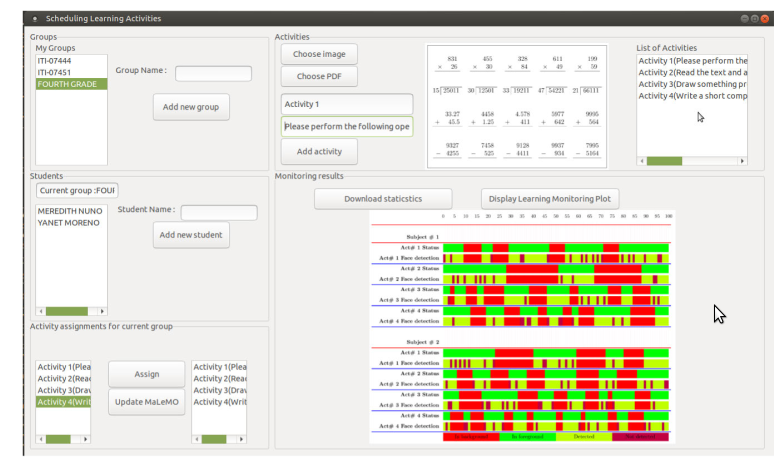
\includegraphics[width=0.95\textwidth]{Figs/LearningMonitoring1}
     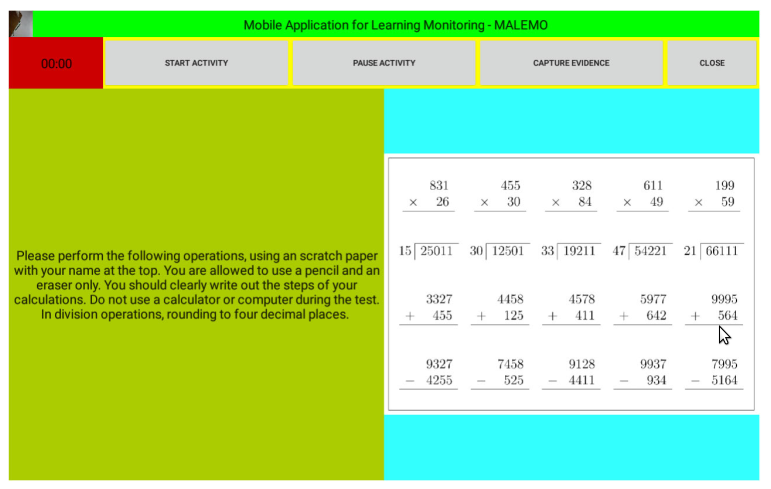
\includegraphics[width=0.95\textwidth]{Figs/LearningMonitoring2}
     \end{center}
\end{column}
\end{columns}


\end{frame}

\begin{frame}{\citetitle{MarcoNuno_Revista_2020_06_00} (3)}


\begin{columns}
\begin{column}{0.5\textwidth}
\begin{block}{Pasos ejecutados por la App: } 
		\begin{itemize}
		\item Detecta la cara del estudiante y estima hacia donde esta mirando (la pantalla, el área de trabajo o el exterior)
		\item Detecta cuando el estudiante cierra la aplicación y lleva la cuenta del tiempo que la aplicación de monitoreo permanece inactiva. 
		\end{itemize}
\end{block} 
	\begin{center}
		 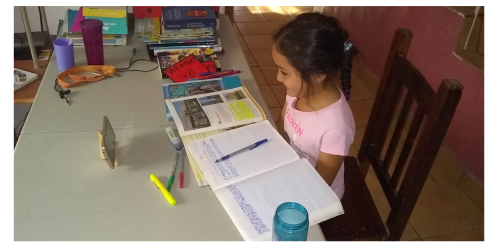
\includegraphics[width=0.50\textwidth]{Figs/LearningMonitoring3}
	\end{center}
\end{column}
\begin{column}{0.5\textwidth}  
    \begin{center}
     %%%%% this is a minipage, so \textwidth is already adjusted to the size of the column
     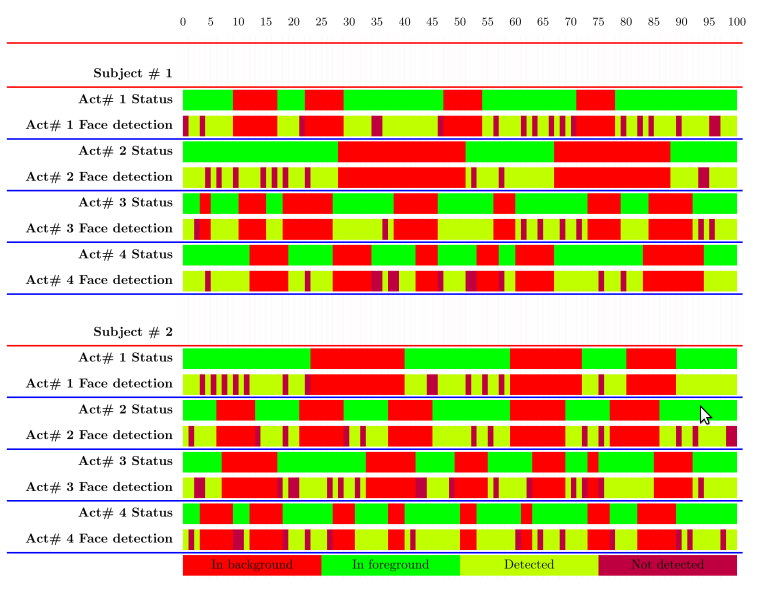
\includegraphics[width=0.99\textwidth]{Figs/LearningMonitoring4}
     \end{center}
\end{column}
\end{columns}

%\end{block} 
\end{frame}


